%!TEX root = optimization1718.tex

\chapter{Early Stoping for Kernel Boosting Algorithms}
\emph{Speaker: Fan Wu and Tomas Vaskevicius}\\


\section{Introduction}
Overfitting is a problem occuring in many models. Especially non-parametric models,
which offer great flexibility, but can also produce very complex models,
are prone to this issue. Usually, some form of regularization has to be introduced
in order to overcome this problem.

Consider a setting where we try to minimize some loss function $\mathcal{L}(f)$
(typically some empirical loss function depending on the observed data) where $f$
can be chosen from some class of functions $\mathcal{H}$. Assuming the
functions are parametrized by some $\theta$, one approach to preventing overfitting
is to add a penalty term (e.g. $||\theta||_2^2$, $||\theta||_1$, a combination of the two etc.)
to the objective function, thus penalizing overly complex models.

In these notes we will present an alternative approach to regularization for kernel boosting algorithms discussed in \cite{wain17ada}. As we will see, instead of penalization regularization one
can consider algorithmic regularization, which can be applied in the form of early stopping
for iterative algorithms. The idea is that if we have some iterative algorithm
converging to a minimizer of the loss function $\mathcal{L}(f)$, this algorithm will
produce a function $f$ fitting well to the observed data but with bad generalization properties
if run until convergence. Instead, the algorithm can be stopped early in order to obtain a regularized estimate.
In particular, in \cite{wain17ada} kernel boosting algorithms are considered
where an optimal stopping time rule is derived which can be computed from the data.

An interesting connection between these two forms of regularization has been shown in
\cite[Section 3.4]{raskutti2014early}.
It has already been observed through simulations that the prediction error behaves
similarly for Kernel Ridge Regression with a penalty parameter and gradient descent algorithms with early stopping, see e.g. \cite{friedman2004gradient}.
\citet{raskutti2014early} provided a theoretical explanation of this observation.
They considered $L^2$ boosting and compared it to KRR.
They showed that the same bounds on the prediction error holds when the same criterion
is applied for the penalty parameter in KRR and the stopping time in the boosting algorithm they consider.

One of the most important advantage of using early stopping as opposed to penalized
regularization forms is lower computational complexity.
As a particular example, when doing kernel ridge regression, for each choice of
regularization parameter we would need to repeatedly perform $\mathcal{O}(n^{3})$
operations where $n$ is the dataset size. On the other hand, using early stopping
with the corresponding gradient algorithm, we would have to perform $\mathcal{O}(Tn^{2})$
operations where $T$ is the computed stopping time.

\section{Kernel Boosting}

Let $\mathcal{H}$ be a Reproducing Kernel Hilbert Space (RKHS) of functions
$f : \mathcal{X} \to \mathbb{R}$ with associated reproducing kernel
$k : \mathcal{X} \times \mathcal{X} \to \mathbb{R}$ so that in particular we have
\begin{align*}
  &\forall x \in \mathcal{X}, k(\cdot, x) \in \mathcal{H} \\
  &\forall x \in \mathcal{X}, \forall f \in \mathcal{H}, \langle f, k(\cdot, x) \rangle_{\mathcal{H}} = f(x).
\end{align*}
Assume we observe some dataset $\{(x_{i}, y_{i}) \mid i = 1, \dots, n\}$
where $x_{i} \in \mathcal{X}$ and $y_{i} \in \mathbb{R}$.
We will treat the covariates $x_{i}$ as fixed an let $y_{i} \sim P_{Y|x_{i}}$.
We then define the population loss functional $\mathcal{L}$ as
$$
\mathcal{L}(f) \coloneqq \mathbb{E}_{Y_{1:n}}\left[ \frac{1}{n} \sum_{i = 1}^{n} \phi(Y_{i}, f(x_{i})) \right]
$$
for some cost function $\phi : \mathbb{R} \times \mathbb{R} \to [0, \infty)$.
Since the population functional at $f$ uses $f$ only at fixed points $x_{1}, \dots, x_{n}$,
by the Representer theorem we know that there exists
$f^{*} \in \mathcal{H}_{n} \coloneqq \text{span}\{k(\cdot, x_{i}) \mid i = 1, \dots, n\}$
minimising $\mathcal{L}$. Since we cannot compute the population loss directly, we will use
empirical loss functional as a proxy:
$$
\mathcal{L}_{n}(f) \coloneqq \frac{1}{n} \sum_{i=1}^{n} \phi(y_{i}, f(x_{i})).
$$

For every $f \in \mathcal{H}_{n}$, we can write $f = \sum_{i = 1}^{n} \alpha_{i} k(\cdot, x_{i})$
where $\alpha_{i} \in \mathbb{R}$.
let $f(x_{1:n})$ denote a column vector in $\mathbb{R}^{n}$ with $i$-th enry
equal to $f(x_{i})$. Let $K$ be an $n \times n$ matrix with $K_{ij} = k(x_{i}, x_{j})$.
Then $f(x_{1:n}) = K \alpha$.
Also, given a vector $z \in \text{range}(K)$, for
$\beta = K^{\dagger}z$
\footnote{$K^{\dagger}$ denotes the generalised inverse of K. That is,
a unique matrix, such that $KK^{\dagger}K = K$},
we have $z = g(x_{1:n})$ and $g = \sum_{i=1}^{n} \beta_{i}k(\cdot, x_{i})$.
Hece, instead of working in $\mathcal{H}_{n}$ we can alternatively work in $\mathbb{R}^{n}$.

We will now derive a formula for applying gradient descent on $\mathbb{R}^{n}$ vectors
of the form $f(x_{1:n})$.
Note that we cannot simply write
$$
f^{t+1}(x_{1:n}) = f^{t}(x_{1:n}) - \alpha_{t} \nabla \mathcal{L}_{n}(f^{t}(x_{1:n}))
$$
because such mapping between $f \in \mathcal{H}_{n}$ and $\mathbb{R}^{n}$ does not
preserve inner products.
To make the $\mathcal{H}_{n}$ and $\mathbb{R}^{n}$ inner products match,
we need to reparameterise our vectors $z \in \text{range}(K)$ as
$\theta_{z} = \sqrt{K^{\dagger}}z$\footnote{
Square roots of positive definite matrices always exist and are unique.
}
so that for $f = \sum_{i=1}^{n} \alpha_{i}k(\cdot, x_{i})$ and  $g = \sum_{i=1}^{n} \beta_{i}k(\cdot, x_{i})$
we have
\begin{align*}
\langle f, g \rangle_{\mathcal{H}_{n}} &= \beta^{T} K \alpha \\
                                         &= \beta^{T} K K^{\dagger} K \alpha \\
                                         &= (\sqrt{K^{\dagger}} K\beta)^{T} (\sqrt{K^{\dagger}} K \alpha) \\
                                         &= \langle \theta_{K\alpha}, \theta_{K\beta} \rangle_{\mathbb{R}^{n}}.
\end{align*}
Hence we can map functions $f = \sum_{i=1}^{n} \alpha_{i}k(\cdot, x_{i})$ to
$\theta_{f} = \sqrt{K^{\dagger}}K\alpha$.
We can now define the loss functino on this reparameterised space as:
$$
\mathcal{J}(\theta_f) = \mathcal{L}_{n}(f(x_{1:n})) = \mathcal{L}_{n}(\sqrt{K}\theta_f).
$$
We can now perform gradient descent on the reprameterised $\mathbb{R}^{n}$ space
as:
\begin{align*}
  \theta_{t+1} &= \theta_{t} - \alpha_{t} \nabla \mathcal{J}(\theta_t) \\
               &= \theta_{t} - \alpha_{t} \sqrt{K} \mathcal{L}_{n}(\sqrt{K}\theta_t).
\end{align*}
Multiplying both sides by $\sqrt{K}$ from the left side (i.e. undoing reparametrisation)
we get
\begin{equation}
  f^{t+1}(x_{1:n}) = f^{t}(x_{1:n}) - \alpha_{t}K\nabla\mathcal{L}_{n}(f^{t}(x_{1:n})
\end{equation}
which will be the gradient descent rule that we are going to work with.

\section{Localised Gaussian Complexity and the Critical Radius}

Recall that our goal is to compute some $T$ before running the kernel boosting
algorithm so that with high probability we have low excess risk:
$$
\mathcal{L}(f^{T}) - \mathcal{L}(f^{*}) \preceq \rho_{n}
$$
where $\rho_{n}$ gets smaller as the dataset size increases.
As a proxy to the excess risk, we can look at the distance
between our estimate $f^{T}$ and the true function $f^{*}$ induced by the empirical
$L_{2}(\mathbb{P}_{n})$ norm $\norm{\cdot}_{n}$ defined as
$$
\norm{f^{T} - f^{*}}_{n} = \frac{1}{n} \sum_{i=1}^{n} (f^{T}(x_{i}) - f^{*}(x_{i}))^{2}.
$$

\subsection{Localised Gaussian Complexity}

Complexity measures such as the Rademacher or Gaussian complexities
are often used to derive generalisation error bounds, see e.g. \cite{bartlett2002rademacher}
and \cite{bartlett2005local}.
The empirical Gaussian complexity is given by
\begin{equation}
  \label{eq:gaussian-complexity}
  \mathcal{G}_{n}(\mathcal{H}) \coloneqq \mathbb{E}_{w_{1:n}}\Big[\sup_{h\in\mathcal{H}}\frac{1}{n}\sum_{i=1}^nw_ih(x_i)\Big],
\end{equation}
where $(w_1,...,w_n)$ is an i.i.d. sequence of $N(0,1)$ random variables.
For i.i.d. $w_{1:n}$ given by $\mathbb{P}(w_i=-1)=\mathbb{P}(w_i=1)=\frac{1}{2}$ the above quantity would
be the Rademacher complexity.
Intuitively, the Equation~\ref{eq:gaussian-complexity} checks how well our class
of hypotheses $\mathcal{H}$ can align with random noise conditionally on the observed data.
The bigger the Gaussian (or Rademacher) complexity, the more complex our function
space $\mathcal{H}$ is, and thus the more likely to overfit the data.
Such complexity measures can be used to derive generalisation error rates
of the order $\mathcal{O}(1/\sqrt{n})$.


As noted in \cite{bartlett2005local}, $\mathcal{G}_{n}(\mathcal{H})$ does not capture the fact
that the algorithm will typically only choose hypotheses from a small subset of the function space
containing functions with small empirical erros. Instead, we can consider local sets of the
form
$$
  \mathcal{E}(\delta):= \{f^{*}-f \mid f\in\mathcal{H}, ||f^{*}-f||_{\mathcal{H}}\le 1, ||f^{*}-f||_n \leq \delta\},
$$
and then consider \textit{localised Gaussian complexities} given by
$\mathcal{G}_{n}(\mathcal{E}(\delta))$. Using these localised complexity measures
faster error rates can be derived. See \citet{bartlett2005local} for more information.

\subsection{Critical Radius}

Let $\sigma$ denote the \textit{noise level} of our data. We follow the definition
given in \citet{wain17ada}:
$$
\sigma \coloneqq
\begin{cases}
  \min\{t \mid \underset{i = 1, \dots, n}{\max} \mathbb{E}[e^{((Y_{i} - f^{*}(x_{i}))^{2}/t^{2}}] \}, & \text{if least squares} \\
  4(2M + 1)(1 + 2C_{\mathcal{H}}), & \text{for } \phi'\text{-bounded losses.}.
\end{cases}
$$
where constants $M$ and $C_{\mathcal{H}}$ will be defined below.

We then define the \textit{critical radius} as the smallest positive number $\delta_{n}$ such that
\begin{equation*}
  \frac{\mathcal{G}_n(\mathcal{E}(\delta_{n}))}{\delta_n} \le \frac{\delta_{n}}{\sigma}
\end{equation*}
which is guaranteed to be unique and exist.

It turns out that the critical radius is a key quantity in relating the quantity
$\norm{f^{T} - f^{*}}_{n}$ to the localised Gaussian complexity.
More information on that is available in scribe lecture notes\footnote{\url{http://www.stat.cmu.edu/~arinaldo/Teaching/36755/F16/Scribed_Lectures/AST_Nov14_Scribe.pdf}} and in a soon to
be published book \citet{wainwright2017high}.

As we shall see later, an optimal stopping rule will be proportional to $\frac{1}{\delta_{n}^{2}}$.
Note that increasing dataset size $n$ will make $\mathcal{G}_{n}(\mathcal{E}(\delta)$ smaller,
so that the critical radius will decrease as the dataset size increases, which will
allow us to run more iterations. Also note, that increasing the noise level $\sigma$
will decrease the critical radius, thus stopping our algorithm earlier to prevent
overfitting.

\subsection{Computing the Critical Radius}

In general, there is no easy way to compute the critical radius.
One of the reasons why we have to restrict ourselves to RKHSs instead of doing
boosting in full generality, is that there are known inequalities able to sandwitch
$\mathcal{G}(\mathcal{E}(\delta))$ by quantities that we can compute from the data.
Define
$$
\mathcal{R}(\delta) \coloneqq \sqrt{\frac{1}{n} \sum_{i=1}^{n} \min(\delta^{2}, \hat{\mu}_{i}}),
$$
where $\hat{\mu}_{i}$ for $i = 1, \dots, n$ are the eigenvalues of the normalised
kernel matrix $\frac{1}{n}K$.
Up to a universal constant, the above value upperbounds $\mathcal{G}_{n}{\mathcal{E}(\delta)}$
for all $\delta \geq 0$. Up to another universal constant it is also a lower bound for all
$\delta \geq \frac{1}{\sqrt{n}}$. In RKHSs case, this will allow us to find the order
of the critical radius.


\section{Main Results}
In this section we will present the main result of \cite{wain17ada}, before which we first introduce some necessary assumptions.
\subsection{Assumptions}
For the main results the following assumptions on the population loss $\mathcal{L}$ will be necessary and always assumed to hold locally (rather than globally, similar to the Gaussian Complexity above). Define $C_{\mathcal{H}}^2 := 2\max\{||f^*||_{\mathcal{H}}^2, 32\}$, then the assumptions have to hold on the ball
\begin{equation}
\mathcal{B}_{\mathcal{H}}(f^*,2C_{\mathcal{H}}) := \{f\in\mathcal{H} \mid ||f-f^*||_{\mathcal{H}} \le 2C_{\mathcal{H}}\},
\end{equation}
where $f^*$ is the population loss minimizer in the Hilbert space $\mathcal{H}$. Choosing $C_{\mathcal{H}}\geq ||f^*||_{\mathcal{H}}$ ensures that we begin in this ball when initializing $f^0=0$.
\begin{itemize}
\item \textbf{m-smooth and M-strongly convex}\\
For all $f,g \in \mathcal{B}_{\mathcal{H}}(f^*,2C_{\mathcal{H}})$,
\begin{equation}
\frac{m}{2}||f-g||_n^2 \le \mathcal{L}(f) - \mathcal{L}(g) - \langle \nabla\mathcal{L}(g), f(x_1^n) - g(x_1^n)\rangle \le \frac{M}{2}||f-g||_n^2,
\end{equation}
where by $\nabla\mathcal{L}(g)$ we mean the vector in $\mathbb{R}^n$ rather than the function in $\mathcal{H}$. In order to show this condition it suffices to (similar to verifying regular convexity) consider the second derivative of the cost function and to show that
\begin{equation*}
m\le \frac{\partial^2\phi(y,\theta)}{\partial\theta^2} \le M
\end{equation*}
holds. This can be seen by considering the Taylor expansion of $\mathcal{L}(f)$. For example, in the case of the least-square cost $\phi(y,\theta)=\frac{(y-\theta)^2}{2}$ this condition can be shown to be satisfied for $m=M=1$. This condition can also be shown to be satisfied for the logistic and the exponential cost.

\item $\mathbf{\phi'-boundedness}$\\
When considering other cost functions than least-squares, we need to further assume that
\begin{equation}
\max_{i=1,...,n}\left\lvert \frac{\partial\phi(y,\theta)}{\partial \theta}\right\rvert_{\theta=f(x_i)} \le B
\end{equation}
for all $f\in \mathcal{B}_{\mathcal{H}}(f^*,C_{\mathcal{H}}^2)$ and $y\in \mathcal{Y}$.

\end{itemize}

Finally, define the \textit{critical radius} $\delta_n$ to be the smallest positive value satisfying
\begin{equation}
\frac{\mathcal{G}_n(\mathcal{E}(\delta_n,1))}{\delta_n} \le \frac{\delta_n}{\sigma},
\end{equation}
where $\sigma$ is the \textit{effective noise level} defined in \cite{wain17ada}.

\subsection{Upper bound on the excess risk and empirical error}
Define the averaged estimator
\begin{equation*}
\bar{f}^T := \frac{1}{T}\sum_{t=1}^T f^t.
\end{equation*}
The following bounds will apply to this averaged estimator rather than the latest element $f^T$, and while numerical experiments suggest that similar results also hold for $f^T$, the proof of the bounds cannot be trivially extended to this case.

\begin{theorem}
\label{thmbound}
(\cite{wain17ada}) Let $\phi$ be a cost function satisfying $\phi'$-boundedness and $\mathcal{L}$ the corresponding population loss function satisfying the m-smooth M-strongly convex condition. Let the sample size $n$ be large enough such that $\delta_n\le \frac{M}{m}$, and $\{f^t\}_{t=1,2,...}$ be functions generated by the iteration REFERENCE using some step size $\alpha\in (0,\min\{\frac{1}{M}, M\}]$ and initialization $f^0=0$. Then, for all iterations $T\in \{0,1,...,\lfloor\frac{m}{8M\delta_n^2}\rfloor$\}, the averaged functions $\bar{f}^T$ satisfies the bounds
\begin{align}
\mathcal{L}(\bar{f}^T) - \mathcal{L}(f^*) &\le \frac{C}{M}\Big(\frac{1}{\alpha m T} + \frac{\delta_n^2}{m^2}\Big), \label{bound1} \\
||\bar{f}^T-f^*||_n^2 &\le C\Big(\frac{1}{\alpha m T} + \frac{\delta_n^2}{m^2}\Big), \label{bound2}
\end{align}
with probability at least $1-c_1\exp\big(-C_2\frac{m^2n\delta_n^2}{\sigma^2}\big)$ (where $c_1$ is a universal constant, and $C$, $C_2$, may depend on the joint distribution and the population loss $\mathcal{L}$).
\end{theorem}

\begin{proof}
We will proof the theorem assuming three technical lemmas, which are stated with the assumptions of theorem \ref{thmbound} in place and for which a proof can be found in \cite{wain17ada}.

Recall that for a function $f\in \mathcal{H}$ we write $\theta_f := f(x_1^n) = (f(x_1),...,f(x_n))\in \mathbb{R}^n$, usually omitting the subscript $f$. Updates on the function values $\theta^t\in \mathbb{R}^n$ correspond uniquely to updates of the functions $f^t\in\mathcal{H}$, so we can consider these instead. For vectors $\Delta\in \operatorname{range}(K)$ we define the Hilbert norm $||\Delta||_{\mathcal{H}}^2 = \frac{1}{n}\Delta^TK^{\dagger}\Delta$ and the empirical norm $||\Delta||_n^2 = \frac{1}{n}||\Delta||_2^2$ (here we abused the notation and used that $\Delta$ can be interpreted both as element in $\mathbb{R}^n$ and in $\mathcal{H}$. We will continue and not make this distinction in the following).

Define $\Delta^t := \theta^t-\theta^*$. The first lemma provides a bound on this error in the empirical norm $||\cdot||_n^2$.\\
\textbf{Lemma 1}
\textit{For any stepsize $\alpha\in(0,\frac{1}{M}]$, we have}
\begin{equation}
\label{lemma1eq}
\frac{m}{2}||\Delta^{t+1}||_n^2\le \frac{1}{2\alpha}(||\Delta^t||_{\mathcal{H}}^2 - ||\Delta^{t+1}||_{\mathcal{H}}^2) + \langle\nabla\mathcal{L}(\theta^*+\Delta^t) - \nabla\mathcal{L}_n(\theta^*+\Delta^t), \Delta^{t+1}|\rangle.
\end{equation}

The second term on the right hand side involves the difference between the gradient of the population and empirical loss, which can be hard to evaluate. The next lemma provides a uniform bound on this term. \\
\textbf{Lemma 2}
\textit{Define}
\begin{equation*}
\mathbb{S} := \{\Delta, \tilde{\Delta}\in \mathbb{R}^n: \Delta,\tilde{\Delta}\in \mathcal{B}_{\mathcal{H}}(f^*,2C_{\mathcal{H}}), ||\Delta||_{\mathcal{H}} \geq 1 \}.
\end{equation*}
\textit{Then, for} $\Delta, \tilde{\Delta} \in \mathbb{S}$,
\begin{equation}
\label{lemma2eq}
\langle\nabla\mathcal{L}(\theta^*+\Delta^t) - \nabla\mathcal{L}_n(\theta^*+\Delta^t), \Delta^{t+1}|\rangle \le 2\delta_n||\Delta||_n + 2\delta_n^2||\Delta||_{\mathcal{H}} + \frac{m}{c_3}||\Delta||_n^2
\end{equation}
\textit{holds with probability at least} $1-c_1\exp(-c_2\frac{m^2n\delta_n^2}{\sigma^2})$.

Since we only made assumptions locally, these bounds naturally only hold when the error iterates are bounded in the Hilbert norm. As noted above with the initialization $f^0=0$ the assumptions apply in the beginning. The next lemma controls the Hilbert norm for subsequent iterations.\\
\textbf{Lemma 3}
\textit{For any step size $\alpha \in (0, \min\{M,\frac{1}{M}\})$ and any iteration $t\le \frac{m}{8M\delta_n^2}$}
\begin{equation}
\label{lemma3eq}
||\Delta^t||_{\mathcal{H}} \le C_{\mathcal{H}}
\end{equation}
\textit{holds with probability at least $1-C_1\exp(-C_2n\delta_n^2)$}

Taking these lemmas as given, we condition on the event that the bounds of the lemmas 2 and 3 hold. Let $t<\frac{m}{8M\delta_n^2}-1$. We first assume that additionally $||\Delta^{t+1}||_n > \delta_n ||\Delta^{t+1}||_{\mathcal{H}}$ holds. Inserting this in (\ref{lemma2eq}) we get
\begin{equation*}
\langle\nabla\mathcal{L}(\theta^*+\Delta^t) - \nabla\mathcal{L}_n(\theta^*+\Delta^t), \Delta^{t+1}\rangle \le 4\delta_n||\Delta^{t+1}||_n + \frac{m}{c_3}||\Delta^{t+1}||_n^2.
\end{equation*}
Substituting this into (\ref{lemma1eq}) we get
\begin{equation*}
\frac{m}{2}||\Delta^{t+1}||_n^2\le \frac{1}{2\alpha}(||\Delta^t||_{\mathcal{H}}^2 - ||\Delta^{t+1}||_{\mathcal{H}}^2) + 4\delta_n||\Delta^{t+1}||_n + \frac{m}{c_3}||\Delta^{t+1}||_n^2.
\end{equation*}

Rearranging and writing $D^t := \frac{1}{2\alpha}(||\Delta^t||_{\mathcal{H}}^2 - ||\Delta^{t+1}||_{\mathcal{H}}^2)$, $\gamma = \frac{1}{2} - \frac{1}{c_3}$ gives
\begin{equation*}
\gamma m ||\Delta^{t+1}||_n^2 \le D^t + 4\delta_n||\Delta^{t+1}||_n,
\end{equation*}
and solving this quadratic equation in $||\Delta^{t+1}||_n^2$ gives
\begin{equation*}
||\Delta^{t+1}||_n^2 \le \frac{c\delta_n^2}{\gamma^2m^2} + \frac{2D^t}{\gamma m}
\end{equation*}
for some universal constant $c$. Now by telescoping this inequality we get
\begin{equation*}
\frac{1}{T}\sum_{t=1}^T||\Delta^t||_n^2 \le \frac{c\delta_n^2}{\gamma^2 m^2} + \frac{1}{T}\sum_{t=1}^T \frac{2D^t}{\gamma m} \le \frac{c\delta_n^2}{\gamma^2 m^2} + \frac{1}{\alpha\gamma m T}(||\Delta^0||_{\mathcal{H}}^2 - ||\Delta^T||_{\mathcal{H}}^2),
\end{equation*}
which (absorbing constants into $C$) gives the same rates as the bounds in the theorem. Recall that we assumed $||\Delta^{t+1}||_n > \delta_n ||\Delta^{t+1}||_{\mathcal{H}}$. If this does not hold, then $||\Delta^{t+1}||_{\mathcal{H}}\le \delta_n ||\Delta^{t+1}||_{\mathcal{H}} \le \delta_n C_{\mathcal{H}}$ by lemma 3, and the above bound holds with the same rates. Finally, by Jensen's inequality we have
\begin{equation*}
||\bar{f}^T - f^*||_n^2 = ||\frac{1}{T}\sum_{t=1}^T \Delta^t||_n^2 \le \frac{1}{T}\sum_{t=1}^T||\Delta^t||_n^2,
\end{equation*}
showing (\ref{bound2}). Finally, (\ref{bound1}) follows by the smoothness assumption:
\begin{equation*}
\mathcal{L}(\bar{f}^T) - \mathcal{L}(f^*) \le \frac{M}{2}|\bar{f}^T - f^*||_n^2
\end{equation*}
\end{proof}
\begin{remark}
Intuitively, the first bound means that (ignoring constants) for iterations $T\le \frac{1}{\delta_n^2}$ the first term $\frac{1}{\alpha m T}$ dominates the second term $\frac{\delta_n^2}{m^2}$. Therefore taking more steps while $T\le \frac{1}{\delta_n^2}$ improves the bound, whereas after that point taking further steps cannot reduce the error bound below the order of $\delta_n^2$. Note that these bounds do not apply for $T\rightarrow \infty$.

In particular, using a step size of $\alpha=\min\{\frac{1}{M}, M\}$ and $T=\frac{m}{8\delta_n^2M}$ we obtain, taking expectations of the second bound,
\begin{equation}
\mathbb{E}||\bar{f}^T-f^*||_n^2 \le C' \frac{\delta_n^2}{m^2},
\end{equation}
which matches the best known bounds for kernel ridge regression; this stresses the parallels between algorithmic regularization realized by early stopping and penalized regularization of kernel ridge regression.
\end{remark}


\subsection{Application in RKHS}
In general, the critical radius $\delta_n$ is hard to find, since both the local Gaussian complexity $\mathcal{G}_n(\mathcal{E}(\delta,1))$ and the effective noise level $\sigma$ are hard to evaluate. However, in an RKHS it is often possible to compute an explicit upper bound for $\delta_n$. Therefore, consider some kernel $k$ with eigenvalues $\mu_j$. In the following we consider two types of decay-conditions on these eigenvalues, under which an upper bound can be obtained.
\begin{itemize}
\item \textbf{$\gamma$-exponential decay} A kernel $k$ satisfies this decay condition if there exist constants $\gamma >0, c_1$ and $c_2$ such that
\begin{equation*}
\mu_j \le c_1 \exp(-c_2 j^{\gamma})
\end{equation*}
holds. Kernels in this class include the Gaussian kernel with Lebesgue measure.
\item \textbf{$\beta$-polynomial decay} This weaker condition holds if a kernels eigenvalues satisfy
\begin{equation*}
\mu_j \le c j^{-2\beta}
\end{equation*}
for some constants $\beta>\frac{1}{2}$ and $c$. Kernels in this class include the Sobolev kernels with Lebesgue measure.
\end{itemize}
Under these eigenvalue conditions, an upper bound for the critical radius can be computed as $\delta_n^2\asymp \frac{(\log n)^{\frac{1}{\gamma}}}{n}$ and $\delta_n^2 \asymp n^{-\frac{2\beta}{2\beta + 1}}$ (up to universal constants) respectively.

In the case of the $\beta$-polynomial decay, let $i$ be the smallest integer with $ci^{-2\beta}\le \delta^2$:
\begin{equation*}
R(\delta) \le \sqrt{\frac{1}{n}\Big(i\delta^2 + c\sum_{j=i+1}^n j^{-2\beta}\Big)}.
\end{equation*}
Plugging in $c\sum_{j=i+1}^n j^{-2\beta}\le c\int_{j=i}^{\infty} j^{-2\beta}dj = \frac{c}{2\beta-1}i^{-2\beta + 1} \le \frac{1}{2\beta-1}i\delta^2$ we get, up to constants,
\begin{equation*}
\sqrt{\frac{i}{n}}\asymp \delta \quad \Leftrightarrow \quad\delta_n^2\asymp n^{-\frac{2\beta}{2\beta+1}}.
\end{equation*}
The case of exponential decay is similar.

Plugging in these values for the critical radius in theorem \ref{thmbound} gives the rates
\begin{equation*}
\mathbb{E}||\bar{f}^T-f^*||_n^2 \le c\begin{cases}
\frac{(\log n)^{\frac{1}{\gamma}}}{n} \quad\text{for $\gamma$-exponential decay}\\
n^{-\frac{2\beta}{2\beta + 1}} \quad\text{for $\beta$-polynomial decay}
\end{cases}
\end{equation*}
\section{Simulations}
Assume we have some data $n$ points $\{x_i\}_{i=1,...,n}$ distributed equidistantly on $[0,1]$. Given these data points, we sample observations $y_i$ according to
\begin{align*}
y_i \sim \operatorname{Bin}(p(x_i), 5), \quad
p(x_i)=\frac{\exp(f^*(x_i))}{1+\exp(f^*(x_i))}, \quad f^*(x) = |x-\frac{1}{2}| - \frac{1}{4}.
\end{align*}

For the estimates of the data-generating function we consider the first-order Sobolev space of Lipschitz functions, which is the RKHS corresponding to the kernel $k(x,x') = 1 + \min(x,x')$. This kernel satisfies the $\beta$-polynomial decay condition with $\beta=1$, indicating the stopping rule $T=cn^{\frac{2}{3}}$.

We consider the logistic cost function $\phi(y,\theta)=\log(1+e^{-y\theta})$. In order to apply theorem \ref{thmbound} we need to verify the conditions on the loss function. The first and second derivatives are
\begin{equation*}
\frac{\partial\phi(y,\theta)}{\partial\theta} = \frac{-ye^{-y\theta}}{1+e^{-y\theta}}, \text{ and } \frac{\partial^2\phi(y,\theta)}{\partial\theta^2} = \frac{y^2}{(e^{-\frac{y\theta}{2}}+e^{\frac{y\theta}{2}})^2}
\end{equation*}
respectively. Clearly, the first derivative is bounded by 1 ($\phi'$-boundedness holds with $B=1$) and the second derivative is bounded from above by $M=\frac{1}{4}$. The an lower bound on the second derivative we have to use the fact that we make the asswumptions only locally. In particular, $\theta=f(x)$ must come from a function $f$ with $||f||_{\mathcal{H}}\le D := C_{\mathcal{H}} + ||f^*||_{\mathcal{H}}$. By the reproducing property we then know that $f(x)|\le MD$ for some constant $M$, and therefore we can lower bound $\frac{\partial^2\phi(y,\theta)}{\partial\theta^2}$ by $m=\frac{1}{e^{MD}+e^{-MD}+2}$.

We initialize the algorithm at $f^0=0$ and run it for a total of $7n$ steps with a constant step size of $\alpha=0.75$. We then compare different stopping times ($T=(2n)^{\kappa}$ for $\kappa=\frac{1}{3},\frac{2}{3},1$) and the oracle gold standard, which chooses the stopping time $G=\operatorname{arg}\min_{t=1,...,2n}||f^t-f^*||_n^2$, that is the best estimate observed during the whole run. For different sample sizes $n$ we run the algorithm 40 times each and average the mean-squared errors.

\begin{figure}
  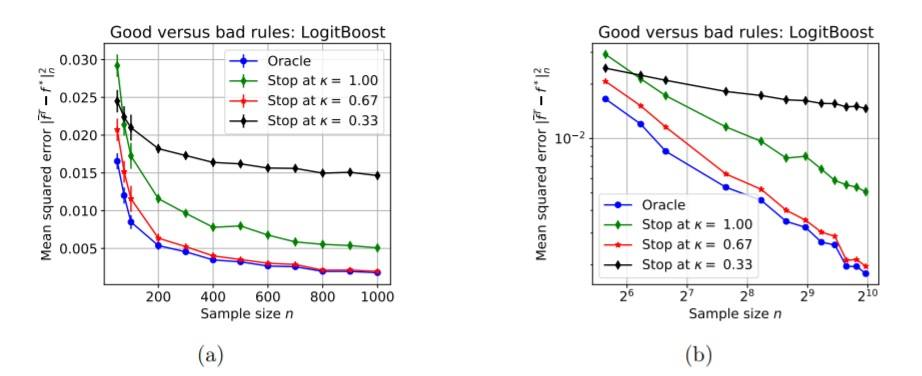
\includegraphics[width=\textwidth]{img/early_stopping_logit_plot.jpg}
  \caption{Illustration taken from \cite{wain17ada}. Mean-squared errors $||\bar{f}^T-f^*||_n^2$ for different stopping rules $T=(7n)^{\kappa}$ and the oracle gold standard (a) and in log-scale (b).}
  \label{l2boost}
\end{figure}

Indeed, the derived stopping rule using $\kappa=\frac{2}{3}$ performs best amongst the early stopping algorithms and has a performance very similar to the oracle gold standard. The slopes in the plot in log-scale confirm the different rates for the error bounds given in theorem \ref{thmbound}.

The two other stopping rules both perform worse. A stopping too early ($\kappa=\frac{1}{3}$) corresponds to underfitting, whereas stopping too late ($\kappa=1$) corresponds to overfitting.

\section{Discussion}
The results of \cite{wain17ada} also show that the derived stopping rule matches a minimax lower bound for a broad class of kernels up to constant factors and is therefore unimprovable. In fact, when stopping at $T=\lfloor \frac{1}{\delta_n^2 \max\{8,M\}}\rfloor$, using a stepsize of $\alpha=\frac{m}{M}$ and initialization $f^0=0$, then for any function $f^*$ with $||f^*||_{\mathcal{H}}\le 1$
\begin{equation}
\mathbb{E}||\bar{f}^T-f^*||_n^2 \asymp \inf_{\hat{f}}\sup_{||f||_{\mathcal{H}}\le 1} \mathbb{E}||\hat{f}-f^*||_n^2.
\end{equation}
Another important aspect of this paper is the role kernels play for these results.
Eigenvalue decay conditions of certain kernels can be used in order to obtain explicit bounds for the critical radius $\delta_n$, which would otherwise be hard to obtain.
Also, we used the the fact that the Hilbert space $\mathcal{H}$ is an RKHS, and that we can therefore restrict our attention to the subspace $\mathcal{H}_n = \operatorname{span}(\{K(\cdot, x_i)\}_{i=1,...,n})$ due to the Representer theorem. This allows us to identify functions in $\mathcal{H}_n$ with vectors in $\mathbb{R}^n$, which is much more convenient to work with.

Finally, throughout these notes we assumed that the covariates $x_{i}$ are fixed.
It is also shown in \citet{wain17ada} that this condition can be relaxed.
Define the $L_{2}(\mathbb{P}_{X})$ norm as $\norm{\cdot}_{2}$ to be given by
$$
\norm{\hat{f} - f^{*}}_{2}^{2} = \mathbb{E}_{X}[(\hat{f}(X) - f^{*}(X))^{2}].
$$
The extension to the random design case work by relating the norms
$\norm{\cdot}_{n}$
and $\norm{\cdot}_{2}$.
In particular, let
$$
\bar{\mathcal{E}}(\delta) \coloneqq \{f^{*}-f \mid f\in\mathcal{H}, ||f^{*}-f||_{\mathcal{H}}\le 1, ||f^{*}-f||_2 \leq \delta\},
$$
and let
\begin{equation}
\bar{\mathcal{G}}_{n}(\bar{\mathcal{E}}(\delta)) \coloneqq
\mathbb{E}_{X_{1:n}, w_{1:n}}\Big[\sup_{h\in\bar{\mathcal{E}}(\delta)}\frac{1}{n}\sum_{i=1}^nw_ih(x_i)\Big],
\end{equation}
where now the expectation is taken also with respect to the covariates.
Let $\bar{\delta}_{n}$ be the identically defined critical radius with respect to
$\bar{\mathcal{G}}_{n}(\bar{\mathcal{E}}(\delta))$.
Then, the difference between the norms
$\norm{\cdot}_{n}$
and $\norm{\cdot}_{2}$ is bounded by a factor proportional to $\bar{\delta}_{n}$
and also $\delta_{n} \leq \bar{\delta}_{n}$. Combining these two facts, we get that
under the same stopping rule $T$, $\norm{\bar{f}^{T} - f^{T}}_{2}^{2} \leq c \bar{\delta}_{n}$
for some constant $c$.

